\documentclass[12pt,a4paper]{article}
\usepackage{graphicx}
\usepackage{fontspec}
\usepackage{geometry}
\geometry{left=1.25in,right=1.25in, top=1in,bottom=1in}
\setmainfont{Arial}
\linespread{1.5}
\usepackage{listings}
\title{24 Hour Project-II}
\author{Yuanyou Yao}
\date{\today}
\begin{document}
\maketitle
\tableofcontents
\section{Introduction}
The purpose of the article is to model the survival of male sparrows (1 = survived, 2 = perished) and physical characteristics of the birds. Belows are explanatory:
\begin{enumerate}
\item{AG} : Ages (1 for adults, 2 for juveniles);
\item{TL} : Total length (mm);
\item{AE} : Alar extent (mm);
\item{WT} : Weight (g);
\item{BH} : Length of beak and head (mm);
\item{HL} : Length of humerus (inch);
\item{FL} : Length of femur (inch);
\item{TT} : Length of tibio-tarsus (inch); 
\item{SK} : Width of skull (inch);
\item{KL} : Length of keel of sternum (inch).
\end{enumerate}
We firstly treat the survival status as \emph{Bernoulli Distribution} and then use \emph{Generalized Linear Regression(GLM)} to find their relationship. In order to find top two fit models, we delete some interactions and use \emph{Stepwise} and the final models are selected by $AIC$ and $BIC$.\\
\newline
After two models are obtained, we perform two test---\emph{Wald Test} and \emph{Likelihood Ratio Test(LRT)}---to verify. More importantly, we are interested in predictivability of models. Therefore, a \emph{repeated random sub-sampling validation} is performed and conclusion can be drawn.\\
\newline
 Accordingly, all R codes are put in the appendix.
\newpage
\section{Methods and Models}
\subsection{Preparation}
\subsubsection{For Response Variable}
Since survival has two status---\emph{Survived} and \emph{Perished}, we use 1 = survived, 2 = perished to show (But in R, we would like to use 0 = perished to satisfy \emph{Logistic Regression Model}).\\ 
\newline
Then we use $\pi_i$ to denote the success probability of $Y_i$ 
\subsubsection{For Explanatory Variable}
There are 55 variables including original ones and interactions. However, because some interactions are dif{}ficult to interpret, we decide to drop them, which are related to the variables KL, SK, TT, FL and HL.\\
\newline
Then, we can do \emph{Logistic Regression}.
\subsection{All Variables Regression}
\subsubsection{Coeffiecients}
We simply do a logistic regression with all variables and get the answer:
\begin{lstlisting}[language = R]
          Coefficients:
                            Estimate 
               (Intercept) 3617.1184
               AG          -138.1104  
               TL           -30.0234
               AE             5.6430 
               WT           -28.1808  
               BH           -95.2689  
               HL            93.3188    
               FL            49.3599   
               TT           -21.0532    
               SK            32.1328   
               KL            39.1353 
               `AG:TL`        0.4236   
               `AG:AE`       -0.6298   
               `AG:WT`        0.6994 
               `AG:BH`        6.5736  
               `TL:AE`        0.0336   
               `TL:WT`       -0.4509    
               `TL:BH`        0.9992    
               `AE:WT`        0.1794    
               `AE:BH`       -0.4686    
               `WT:BH`        1.7102  
\end{lstlisting}
\subsubsection{Outliers and Influntial Observations}
We initially check whether the model has any outliers or influntial observations. To begin with, we check studentized residuals and get the following graph:
\newline
\begin{center}
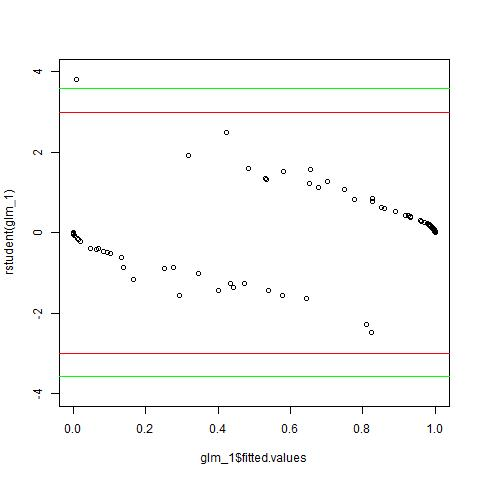
\includegraphics[scale = 0.6]{rstudent.jpg}
\end{center}
By rule of thumb: $\vert t_i \vert > t_{n - p - 1, 1 - \frac{\alpha}{2n}}$, the figure tells us that $NO.3$  $Y$ is an outlier. So, it should be deleted.\\
\newline
Besides, we check influntial observations using \emph{cook's distance} and get the following graph:
\newline
\begin{center}
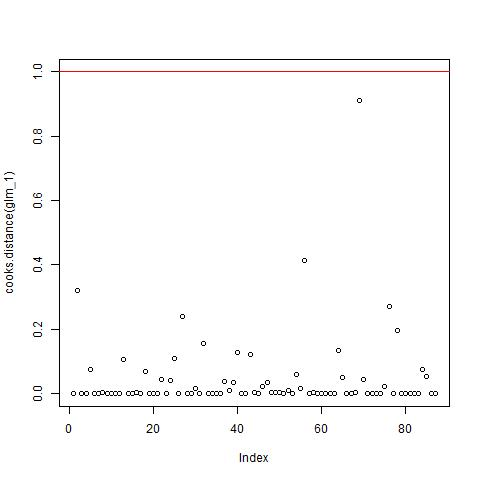
\includegraphics[scale = 0.6]{cook.jpg}
\end{center}
Based on the image,we can say that there are no influntial observations. 
\subsection{Stepwise Selection: Forward Model}
\subsubsection{Model}
Based on the model in 2.2 and $3^{rd}$ observation has been dropped, forward selection is applied to find best model. According to R, we get two models based on $AIC$ and $BIC$.
\[AIC : Status = 53.54683 - 0.71944TL + 58.16916HL - 0.90114WT + 23.76916KL +\]\[ 0.00291AE*BH\]
\[BIC : Status = 49.1871 - 0.6492TL + 72.0453HL - 0.7942WT + 27.1529KL\]
\subsubsection{Tests}
Then we consider AUCs:
\begin{center}
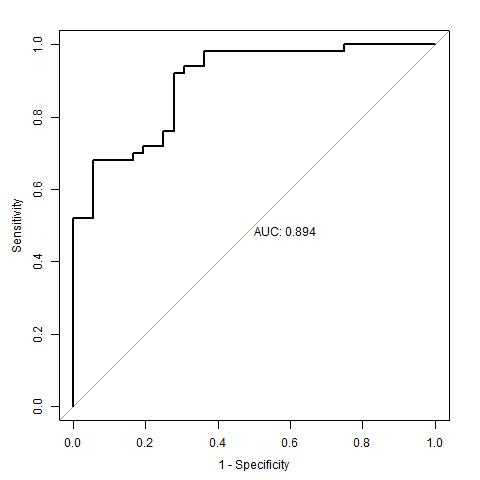
\includegraphics[scale = 0.4]{forwardA.jpg}
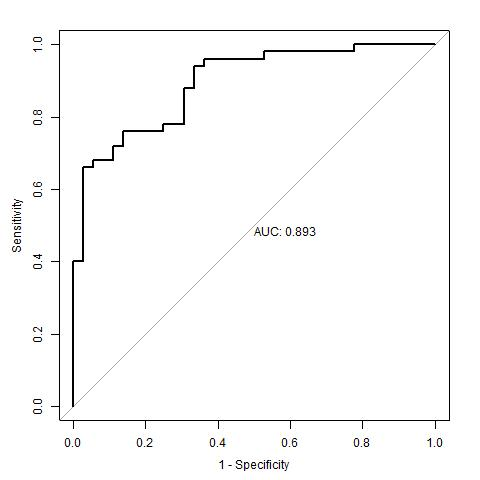
\includegraphics[scale = 0.4]{forwardB.jpg}
\end{center}
Thus, we choose the first model as one of the best models $i.e.$
\[Status = 53.54683 - 0.71944TL + 58.16916HL - 0.90114WT + 23.76916KL +\]\[ 0.00291AE*BH\]
Generally, AUC is $0.894$ and we can interpret it as excellent discrimination\\
\newline
In addition, \emph{Wald Test} and \emph{Likelihood Ratio Test(LRT)} are performed to ensure the model is valid. Belows are some of the result from R:
\begin{center}
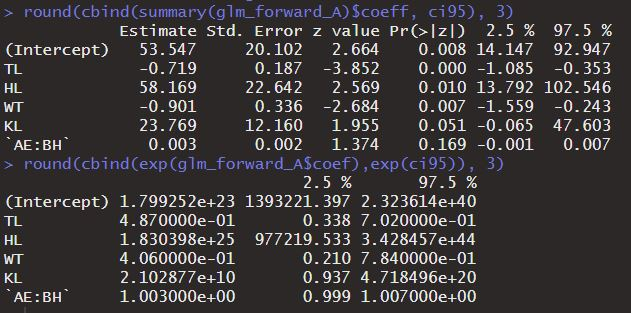
\includegraphics[scale = 0.6]{wald.jpg}
\end{center}
\begin{lstlisting}[language = R]
> Anova(glm_forward_A, type="III")
Analysis of Deviance Table (Type III tests)

Response: y
        LR Chisq Df Pr(>Chisq)    
TL       25.6980  1  3.992e-07 ***
HL        8.1424  1   0.004324 ** 
WT        9.5551  1   0.001994 ** 
KL        4.4056  1   0.035822 *  
`AE:BH`   2.0003  1   0.157264    
---
Signif. codes:  0 ‘***’ 0.001 ‘**’ 0.01 ‘*’ 0.05 ‘.’ 0.1 ‘ ’ 1
\end{lstlisting}
As we can see, the model selected above satisfies the tests well. 
\subsubsection{Interpretation}
We consider the first observation, which is:	
\begin{center}
\begin{tabular}{|l|l|l|l|l|l|}
\hline
Intercept & TL  & HL   & WT   & KL   & $AE*BH$ \\ \hline
1         & 154 & 0.69 & 24.5 & 0.83 & 7519.2  \\ \hline
\end{tabular}
\end{center}
Then we get the success probability \[\pi_1 = \frac{exp(X^T\hat{\beta})}{1+exp(X^T\hat{\beta})} = 0.7147148\]
When these variables are fixed, the probability that the sparrows survive is $\pi_1 = 0.7147148$\\
\newline
We think about the coefficients of TL, which $\beta_1 = -0.71944$. Consider $exp(\beta_1) = 0.4870226$ and it is called \emph{odd ratio}. It means that given other varibles fixed, when total length be 1 mm longer, sparrows are more likely to die during the winter storm. The probability they will survive will be $0.4870226 * 0.7147148 = 0.3480823$.
\subsection{Stepwise Selection: Backward Model}
\subsubsection{Model}
Based on the model in 2.2 and $3^{rd}$ observation has been dropped, backward selection is applied to find best model. According to R, both $AIC$ and $BIC$ find the same model which is:
\[Status = 165.323559 - 1.649037TL - 3.814491BH + 72.846849HL + 34.281506KL -\]
 \[0.458239AG*AE + 3.594124AG*BH + 0.004119TL*AE - 0.006282TL*WT\]
\subsubsection{Tests}
At first we check AUC:
\begin{center}
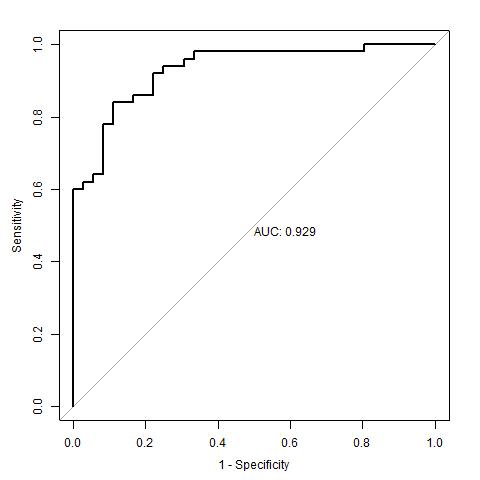
\includegraphics[scale = 0.6]{backward.jpg}
\end{center}
Generally, AUC is $0.929$ and we can interpret it as outstanding discrimination.\\
\newline
In addition, \emph{Wald Test} and \emph{Likelihood Ratio Test(LRT)} are performed to ensure the model is valid. Belows are some of the result from R:
\begin{center}
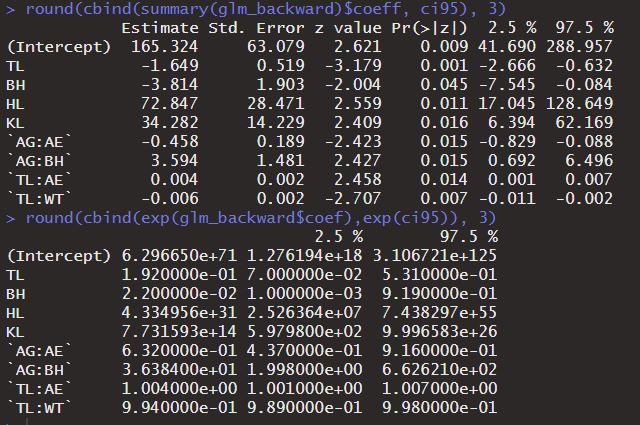
\includegraphics[scale = 0.6]{waldB.jpg}
\end{center}
\begin{lstlisting}[language = R]
> Anova(glm_backward, type="III")
Analysis of Deviance Table (Type III tests)

Response: y
        LR Chisq Df Pr(>Chisq)    
TL       14.9124  1  0.0001126 ***
BH        5.1889  1  0.0227317 *  
HL        8.1407  1  0.0043283 ** 
KL        7.3669  1  0.0066434 ** 
`AG:AE`   8.9230  1  0.0028160 ** 
`AG:BH`   8.9525  1  0.0027709 ** 
`TL:AE`   8.1827  1  0.0042291 ** 
`TL:WT`  10.3317  1  0.0013076 ** 
---
Signif. codes:  0 ‘***’ 0.001 ‘**’ 0.01 ‘*’ 0.05 ‘.’ 0.1 ‘ ’ 1
\end{lstlisting}
As we can see, the model selected above satisfies the tests well. 
\subsubsection{Interpretation}
We consider the first observation, which is:	
\begin{center}
\begin{tabular}{|l|l|l|l|l|l|l|l|l|}
\hline
Intercept & TL  & GH   & HL   & KL   & $AG*AE$ & $AG*BH$ & $TL*AE$ & $TL*WT$ \\ \hline
1         & 154 & 31.2 & 0.69 & 0.83 & 241     & 31.2    & 37114   & 3773    \\ \hline
\end{tabular}
\end{center}
Then we get the success probability \[\pi_1 = \frac{exp(X^T\hat{\beta})}{1+exp(X^T\hat{\beta})} = 0.7055035 \]
When these variables are fixed, the probability that the sparrows survive is $\pi_1 = 0.7055035 $\\
\newline
We think about the coefficients of TL, which $\beta_1 = -1.649037$. Consider $exp(\beta_1) = 0.1922349$ and it is called \emph{odd ratio}. It means that given other varibles fixed, when total length be 1 mm longer, sparrows are more likely to die during the winter storm. The probability they will survive will be $0.1922349 * 0.7055035 = 0.1356224$.
\section{Results}
To campare the predictability of two models above, \emph{cross validation} can be applied. Belows are the main steps:
\begin{enumerate}
\item Split the data into 2 parts and name as train and test. The proportion used of train and test sample is .75.
\item Use the explanatory variables in 2.3 and 2.4 to do GLM with trained data, and use test data for prediction.
\item Record the 2 Area Under the ROC Curve (AUC). 
\item Repeat (1) to (3) for 500 times. Calculate the mean AUCs and compare the two numbers.
\end{enumerate}
Here is what we get:
\[AUC.forward = 0.8462902\]
\[AUC.backward = 0.8822151\]
Consequently, we get the best model:
\[Status = 165.323559 - 1.649037TL - 3.814491BH + 72.846849HL + 34.281506KL -\]
 \[0.458239AG*AE + 3.594124AG*BH + 0.004119TL*AE - 0.006282TL*WT\]
\section{Limitations}
\begin{enumerate}
\item There must be some useful interactions for us to predict but we arbitrarily delete them. For example, $TT*SK$ means the product of tibio-tarsus and skull length, which could an significant level to evaluate the stamina of sparrows to find food in a storm and contribute them to survive. As a consequence, our model cannot reflect all aspects that survival is related.
\item As for original data, we check outliers and influntial observations. It is neccessary to notice that we use \emph{standardized residuals} and \emph{student residuals} to check outliers and \emph{DFFITS}, \emph{cook's distance} and \emph{DFBETAS} to check observation. However, these methods give dif{}ferent results that will be attached in appendix. In our analysis, we just use one to decide whether the obsevations should be drop or not. If we use other methods, which will delete more according to calculation, the final model can be more convincing.
\item It can be infer from 2.3.2, while doing LRT, the p-value of variable $AE*BH$ is $0.157264$.So it is not as good as the model in 2.4.1. Correspondently, the predictability support our assertion.
\end{enumerate}
\section{Conclusions}
In the report, we propose top two models that is used to find how survival is related to physical characteristics. Initially, we use the whole data to do \emph{logistic regression} and check the validation of data. After deleting some influtial observations, we then conduct \emph{stepwise selection} to reduce the variables. Finally, we get two models that satisfy our requirement by \emph{wald test} and\emph{LRT}. A \emph{cross validation} is performed to reach the goal of predictability and we have the best model:
\[Status = 165.323559 - 1.649037TL - 3.814491BH + 72.846849HL + 34.281506KL -\]
 \[0.458239AG*AE + 3.594124AG*BH + 0.004119TL*AE - 0.006282TL*WT\]
When choose the best-fit models, we give some interpretations about coefficients and some details concerning to tests have been mentioned as well.\\
\newline
We also look back the whole analysis and find some critical issuses like dropped variables that can change the final models to a considerable degree.
\appendix
\section{Appendix R Code}
\begin{lstlisting}[language =R]
library(car)
library(bestglm)
data=read.csv("24H_project2.csv",header = T,
stringsAsFactors = F)
data$Status[data$Status=="Survived"]=1
data$Status[data$Status=="Perished"]=0
data$Status=as.numeric(data$Status)
table(data$Status)
prop.table(table(data$Status))
f <- as.formula(y ~ .*.)
y <- data$Status
x <- model.matrix(f, data[,-1])[, -1]
x=x[,-c(54,53,50,47,43,38,32,25,17,55,54,52,51,48,49,45,
44,40,39,34,33,26,27,19,18,15,16,23,24,30,31,37,36,41,42,
46,47,50)]
data_new=as.data.frame(cbind(y,x))
attach(data_new)
glm_1=glm(y~.,data = data_new,family = binomial("logit"))
summary(glm_1)
jpeg("glm_1.jpg")
par(mfrow=c(2,2), pty="s")
plot(glm_1)
dev.off()
cbind(resid(glm_1),rstandard(glm_1),rstudent(glm_1))
plot(glm_1, which=3)
plot(glm_1$fitted.values,sqrt(abs(rstandard(glm_1))), 
ylim=c(0,1.5))
plot(glm_1$fitted.values,rstandard(glm_1))
# check studentized residuals
jpeg("rstudent.jpg")
plot(glm_1$fitted.values,rstudent(glm_1), ylim=c(-4,4))
abline(h=c(-3,3), col="red")
# Bonferroni correction
alpha <- 0.05
t.critical <-qt(1-alpha/(2*n), n-p-1)
abline(h=c(-t.critical, t.critical), col="green")
dev.off()
glm_1$fitted.values[max(rstudent(glm_1))]
# Identifying Influential Observations# 
dffits(glm_1)
plot(dffits(glm_1))
abline(h=1, col="red")
# Cook's distance
cooks.distance(glm_1)
plot(glm_1, which = 4)
jpeg("cook.jpg")
plot(cooks.distance(glm_1),ylim = c(0,1))
abline(h=1, col="red")
dev.off()
# DFBETAS
dfbetas(glm_1)
plot(dfbetas(glm_1)[,2])# DFBETAS_{1(i)}
abline(h=1, col="red")
data_new=data_new[-3,]
y=data_new$y
glm_1=glm(y~.,data = data_new,family = binomial("logit"))
step(glm_1,k=log(length(y)))#backward+BIC
step(glm_1)#backward+AIC
if(!require("pROC")) {
  install.packages("pROC")
  stopifnot(require("pROC"))}
glm_backward=glm(formula = y ~ TL + BH + HL + KL + `AG:AE` +
 `AG:BH` + `TL:AE` +  `TL:WT`, family = binomial("logit"),
 data = data_new)
backward.pROC <-roc(y~ fitted(glm_backward))
jpeg("backward.jpg")
plot.roc(backward.pROC, legacy.axes=TRUE, print.auc=TRUE)
dev.off()
ci95 <-confint.default(glm_backward)
round(cbind(summary(glm_backward)$coeff, ci95), 3)
round(cbind(exp(glm_backward$coef),exp(ci95)), 3)
Anova(glm_backward, type="III")
attach(data_new)
glm0 <-glm(y~1, family=binomial("logit"))
step(glm0, scope =list(upper=glm_1), 
direction = "forward")#forward+AIC
step(glm0,scope = list(upper=glm_1),direction = "forward",
k=log(length(y)))#forward+BIC
glm_forward_A=glm(formula = y ~ TL + HL + WT + KL+`AE:BH`, 
family = binomial("logit"), data = data_new)
glm_forward_B=glm(formula = y ~ TL + HL + WT + KL, 
family = binomial("logit"), data = data_new)
forward.pROC.A <-roc(y~ fitted(glm_forward_A))
forward.pROC.B <-roc(y~ fitted(glm_forward_B))
jpeg("forwardA.jpg")
plot.roc(forward.pROC.A, legacy.axes=TRUE, print.auc=TRUE)
dev.off()
jpeg("forwardB.jpg")
plot.roc(forward.pROC.B, legacy.axes=TRUE, print.auc=TRUE)
dev.off()
ci95 <-confint.default(glm_forward_A)
round(cbind(summary(glm_forward_A)$coeff, ci95), 3)
round(cbind(exp(glm_forward_A$coef),exp(ci95)), 3)
Anova(glm_forward_A, type="III")
model1.auc=vector()
model2.auc=vector()
for (i in 1:500) {
p <- 0.75 # ratio btw train vs. valid, which you can decide
idx <-sample.int(n = nrow(data_new),
 size = floor(p*nrow(data_new)),replace = FALSE)
train_data <- data_new[idx,]
test_data <- data_new[-idx,]
#Fit the two models with train data.

model1.trained <- glm(formula = y ~ TL + HL + WT + 
KL +AE*BH, family = binomial("logit"), data=train_data)
model2.trained <- glm(formula = y ~ TL + BH + HL + KL +
 `AG:AE` + `AG:BH` + `TL:AE` +  `TL:WT`, 
family = binomial("logit"), data=train_data)
#Predict your response with validation data.

model1.pred <- predict.glm(model1.trained,
 newdata = test_data, type="response")
model2.pred <- predict.glm(model2.trained,
 newdata = test_data, type="response")

#Compute the AUC and record it 
#(because we will repeat this 500 times).

if (!require("pROC")) {
  install.packages("pROC")
  stopifnot(require("pROC"))
}
model1.auc[i] <- auc(roc(test_data$y, model1.pred))[[1]] 
model2.auc[i] <- auc(roc(test_data$y, model2.pred))[[1]] 
#Repeat a) to d) 500 hundred times
# and record your AUCs, and then average.
}
(model1.ave=mean(model1.auc))
(model2.ave=mean(model2.auc))
\end{lstlisting}
\newpage
\section{Output of R}
\begin{center}
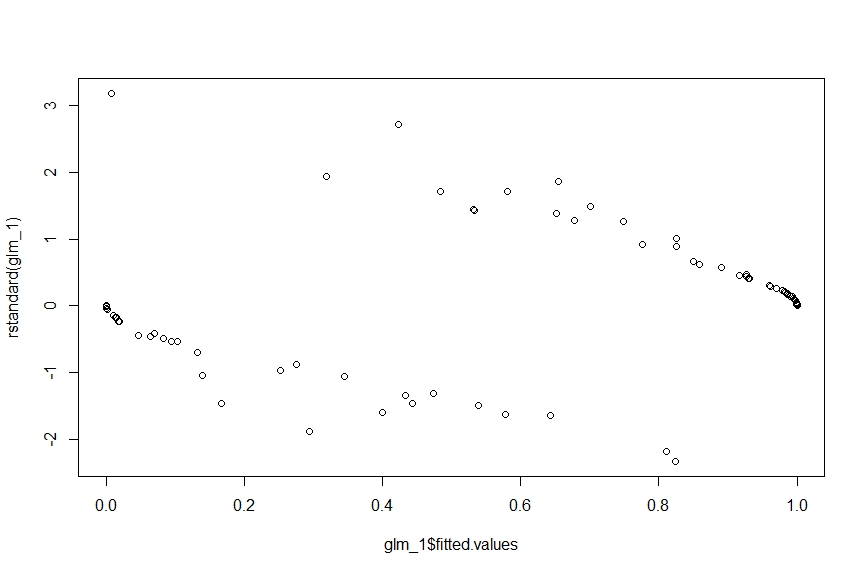
\includegraphics[scale = 0.6]{rstandard.jpeg}
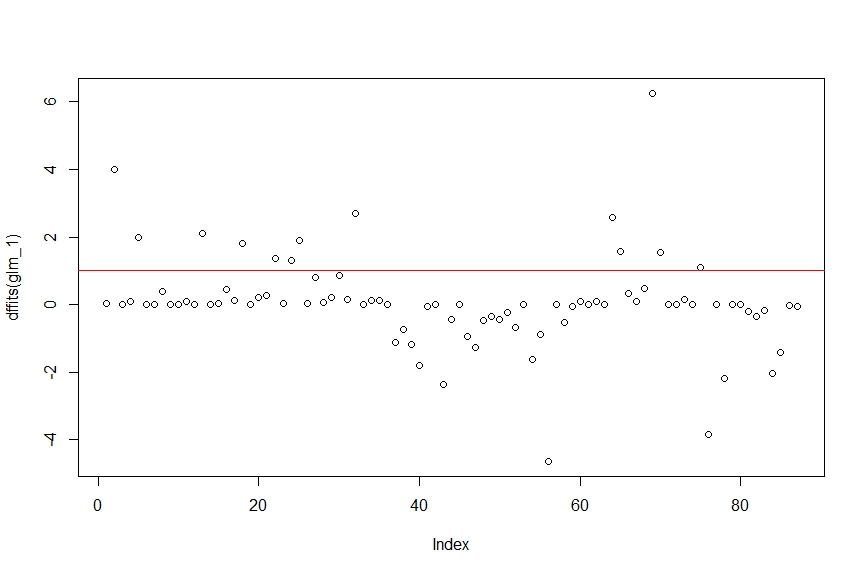
\includegraphics[scale = 0.6]{DFFITS.jpeg}
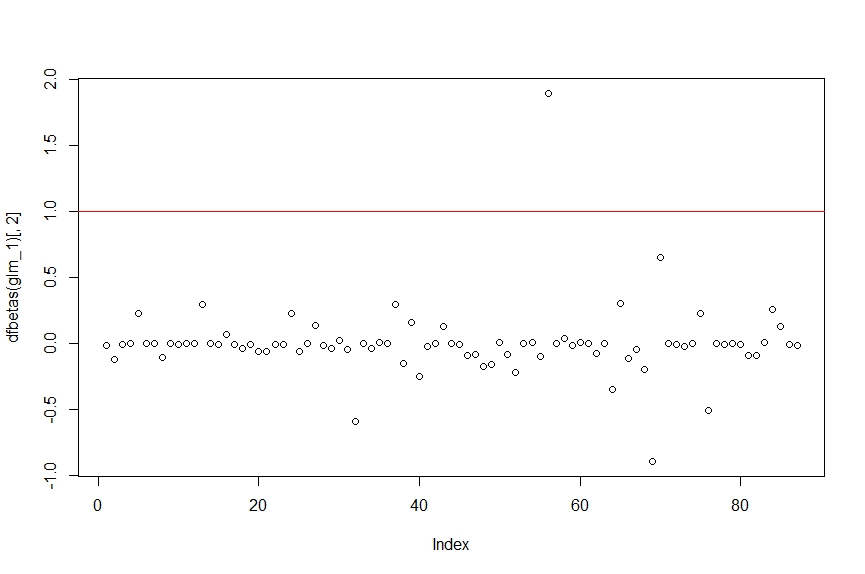
\includegraphics[scale = 0.6]{DFBETAS.jpeg}
\end{center}
\end{document}
